\documentclass{article}
\usepackage{import}
\subimport*{./}{macro}
\usepackage[normalem]{ulem}

\setlength\parindent{0px}

\begin{document}
\setcounter{aprob}{0}
\setcounter{bprob}{0}
\title{Homework \#0}
\author{
    \normalsize{CSEP 546: Machine Learning}\\
    \normalsize{Professor Jamie Morgenstern}\\
    \normalsize{Due: \textbf{\sout{Wednesday April 8, 2026 11:59pm} \; Updated: Thursday April 9, 2026 6:25pm (just before class)}}\\
    \normalsize{38 points}
}
\date{{}}
\maketitle

\section*{Probability and Statistics}
\begin{aprob}
    \points{2} (From Murphy Exercise 2.4.) 
    After your yearly checkup, the doctor has bad news and good news. 
    The bad news is that you tested positive for a serious disease, and that the test is 99\% accurate (i.e., the probability of testing positive given that you have the disease is 0.99, as is the probability of testing negative given that you don't have the disease).
    The good news is that this is a rare disease, striking only one in 10,000 people.
    What are the chances that you actually have the disease?
    
    \subsubsection*{What to Submit:}
    \begin{itemize}
        \item Final Answer
        \item Corresponding Calculations
    \end{itemize}

    \subsubsection*{Solution:}

    \textbf{Known Information:}
    The disease is extremely rare (1 in 10,000), so a 99\% accurate test will produce ${\sim}101$ positive tests out of 10,000 people, of which only 1 person actually has the disease---meaning 1 true positive and 100 false positives.

    Therefore, the total probability of testing positive comes from two groups: people with the disease who test positive + people without the disease who test positive.

    \medskip
    \textbf{Definitions:}
    \begin{itemize}
        \item Hypothesis $H$: you have the disease
        \item Prior: $P(H) = \frac{1}{10{,}000} = 0.0001$ \quad (rate of the disease in the population)
        \item $P(E \mid H) = 0.99$ \quad (true positive: test is positive given you have the disease)
        \item $P(E \mid \neg H) = 0.01$ \quad (false positive: test is positive given you don't have the disease)
    \end{itemize}

    \medskip
    \textbf{Step 1: Compute $P(E)$} --- the probability of testing positive across the entire population.

    This is the sum of:
    \begin{itemize}
        \item People with disease testing positive: $P(E \mid H) \cdot P(H)$
        \item People with no disease testing positive: $P(E \mid \neg H) \cdot P(\neg H)$
    \end{itemize}

    \begin{align*}
        P(E) &= P(E \mid H) \cdot P(H) + P(E \mid \neg H) \cdot P(\neg H) \\
              &= (0.99)(0.0001) + (0.01)(0.9999) \\
              &= 0.000099 + 0.009999 \\
              &= 0.010098
    \end{align*}

    \medskip
    \textbf{Step 2: Apply Bayes' Theorem} --- of all the people who tested positive, what fraction truly have the disease.

    \begin{align*}
        P(H \mid E) &= \frac{P(E \mid H) \cdot P(H)}{P(E)} \\[6pt]
                     &= \frac{(0.99)(0.0001)}{0.010098} \\[6pt]
                     &= \frac{0.000099}{0.010098} \\[6pt]
                     &= 0.00980392156
    \end{align*}

    \medskip
    \textbf{Final Answer:} $P(H \mid E) \approx 0.9804\%$

    \medskip
    \textbf{Collaboration:} \texttt{hw0/chat\_conversation\_export\_A1.md} in Appendix section.

\end{aprob}

\noindent\rule{\textwidth}{0.4pt}

\clearpage{}
\begin{aprob}
    Let $\mathbf{X} = \begin{bmatrix}
        X_1 & \cdots & X_n
    \end{bmatrix}^\top$ be a random vector with mean vector $\boldsymbol{\mu} \in \R^n$ and covariance matrix $\boldsymbol\Sigma \in \R^{n \times n}$. That is, for each $i \in [n]$, $\E {X_i} =\boldsymbol\mu_i$, and for each $i,j \in [n]$, $\Cov{X_i}{X_j} = \boldsymbol\Sigma_{i,j}$.
    \begin{enumerate}
        \item \points{2} Let $i \in [n]$. Find an expression for $\E{X_i^2}$ in terms of only $\boldsymbol\mu$ and $\boldsymbol\Sigma$.
        \item \points{2} Recall that the trace of a square matrix is the sum of its diagonal entries. Show that $\E{\mathbf{X}^\top \mathbf{X}} = \mathrm{tr}(\boldsymbol\Sigma) + \boldsymbol\mu^\top\boldsymbol\mu$. \\
    \end{enumerate}

    \subsubsection*{What to Submit:}
    \begin{itemize}
        \item \textbf{Part a:} Expression for $\E{X_i^2}$ and corresponding calculations
        \item \textbf{Part b:} Proof
    \end{itemize}

    \subsubsection*{Solution:}

    \begin{mdframed}
    \textbf{\large Part a:} Find an expression for $\E{X_i^2}$
    \end{mdframed}

    \textbf{Known Information:}
    \begin{itemize}
        \item $\mathbf{X} = [X_1, \ldots, X_n]^\top$ is a random vector
        \item $\E{X_i} = \boldsymbol\mu_i$ (mean of the $i$-th dimension/feature)
        \item $\Cov{X_i}{X_j} = \boldsymbol\Sigma_{i,j}$ (covariance matrix entry)
        \item From this we can deduce: $\Var{X_i} = \boldsymbol\Sigma_{i,i}$ (diagonal entries = variances, i.e.\ $i = j$)
    \end{itemize}

    \medskip
    \textbf{Definitions:}
    \begin{itemize}
        \item Variance is the expected value of the squared deviation from the mean $\boldsymbol\mu$ of a random variable:
        \[
            \Var{X} = \E{(X - \mu)^2}
        \]
        \item When $c$ is a scalar/constant: $\E{c} = c$ and $\E{cX} = c\,\E{X}$
        \item And $\mu = \E{X}$
    \end{itemize}

    \medskip
    \textbf{Step 1:} Relation between $\mu$ and variance.
    \begin{align*}
        \Var{X} &= \E{(X - \mu)^2} \\
                &= \E{X^2 - 2X\mu + \mu^2} \\
                &= \E{X^2} - \E{2X\mu} + \E{\mu^2}
    \end{align*}

    \textbf{Step 2:} $2$ and $\mu$ are constants and $\E{c} = c$; replace constants and simplify.
    \begin{align*}
        \Var{X} &= \E{X^2} - 2\mu\,\E{X} + \mu^2 \\
                &= \E{X^2} - 2\mu^2 + \mu^2 \\
                &= \E{X^2} - \mu^2
    \end{align*}

    Therefore:
    \begin{align*}
        \boldsymbol\Sigma_{i,i} &= \E{X_i^2} - \boldsymbol\mu_i^2 \\
        \E{X_i^2} &= \boldsymbol\Sigma_{i,i} + \boldsymbol\mu_i^2
    \end{align*}

    \medskip
    \textbf{Final Answer:} $\boxed{\E{X_i^2} = \boldsymbol\Sigma_{i,i} + \boldsymbol\mu_i^2}$

    \bigskip
    \begin{mdframed}
    \textbf{\large Part b:} Show that $\E{\mathbf{X}^\top \mathbf{X}} = \mathrm{tr}(\boldsymbol\Sigma) + \boldsymbol\mu^\top\boldsymbol\mu$
    \end{mdframed}

    $\mathbf{X} = [X_1, \ldots, X_n]^\top$ is a random vector, so its dot product is:
    \[
        \mathbf{X}^\top \mathbf{X} = X_1^2 + X_2^2 + X_3^2 + \cdots + X_n^2
    \]

    Expectation on the right-hand side can be written as a sum of individual expectations:
    \[
        \E{\mathbf{X}^\top \mathbf{X}} = \E{X_1^2} + \E{X_2^2} + \E{X_3^2} + \cdots + \E{X_n^2}
    \]

    Now replace using the relation derived in Part a:
    \begin{align*}
        \E{\mathbf{X}^\top \mathbf{X}} &= (\boldsymbol\Sigma_{1,1} + \boldsymbol\mu_1^2) + (\boldsymbol\Sigma_{2,2} + \boldsymbol\mu_2^2) + (\boldsymbol\Sigma_{3,3} + \boldsymbol\mu_3^2) + \cdots + (\boldsymbol\Sigma_{n,n} + \boldsymbol\mu_n^2) \\
        &= (\boldsymbol\Sigma_{1,1} + \boldsymbol\Sigma_{2,2} + \boldsymbol\Sigma_{3,3} + \cdots + \boldsymbol\Sigma_{n,n}) + (\boldsymbol\mu_1^2 + \boldsymbol\mu_2^2 + \boldsymbol\mu_3^2 + \cdots + \boldsymbol\mu_n^2)
    \end{align*}

    \begin{itemize}
        \item $(\boldsymbol\Sigma_{1,1} + \boldsymbol\Sigma_{2,2} + \boldsymbol\Sigma_{3,3} + \cdots + \boldsymbol\Sigma_{n,n})$ is the trace of the covariance matrix $= \mathrm{tr}(\boldsymbol\Sigma)$
        \item $(\boldsymbol\mu_1^2 + \boldsymbol\mu_2^2 + \boldsymbol\mu_3^2 + \cdots + \boldsymbol\mu_n^2)$ is the dot product $= \boldsymbol\mu^\top \boldsymbol\mu$
    \end{itemize}

    \medskip
    \textbf{Final Answer:} $\boxed{\E{\mathbf{X}^\top \mathbf{X}} = \mathrm{tr}(\boldsymbol\Sigma) + \boldsymbol\mu^\top \boldsymbol\mu}$ \qed

    \medskip
    \textbf{Collaboration:} \texttt{hw0/covariance\_matrix\_conversation\_A2.md} in Appendix section.

\end{aprob}

\noindent\rule{\textwidth}{0.4pt}

\clearpage{}
\begin{aprob}
    Let $X_1, X_2, ..., X_n \sim \mathcal{N}(\mu, \sigma^2)$ be i.i.d. random variables. Compute the following:
    \begin{enumerate}
        \item \points{1} $a\in{\mathbb R},b\in{\mathbb R}$ such that $aX_1+b \sim \mathcal{N}(0,1)$.
        \item \points{2} Using $a$ and $b$ from the previous part, $\E{|aX_1+b|}$.\\ \textbf{Hint:} You may need to use u-substitution.
        \item \points{1} $\E{X_1 + 2X_2}, \Var{X_1 + 2X_2}$.
        \item \points{2} Setting $\widehat{\mu}_n = \frac{1}{n} \sum_{i=1}^n X_i$, the mean and variance of $\sqrt{n}(\widehat{\mu}_n - \mu)$.
    \end{enumerate}

    \subsubsection*{What to Submit:}
    \begin{itemize}
        \item \textbf{Part a:} $a$, $b$
        \item \textbf{Part b:} $\E{|aX_1+b|}$
        \item \textbf{Part c:} $\E{X_1 + 2X_2}$, $\Var{X_1 + 2X_2}$
        \item \textbf{Part d:} $\E{\sqrt{n}(\widehat{\mu}_n - \mu)}$, $\Var{\sqrt{n}(\widehat{\mu}_n - \mu)}$
        \item \textbf{Parts a-d} Corresponding calculations
    \end{itemize}

    \subsubsection*{Solution:}

    \begin{mdframed}
    \textbf{\large Part a:} Find $a, b \in \mathbb{R}$ such that $aX_1 + b \sim \mathcal{N}(0,1)$
    \end{mdframed}

    \textbf{Known:}
    \begin{itemize}
        \item $X_1, X_2, \ldots, X_n \sim \mathcal{N}(\mu, \sigma^2)$ i.i.d.
        \item $\mathcal{N}(0, 1) \Rightarrow \mu = 0,\; \sigma^2 = 1$
        \item $X_1 \sim \mathcal{N}(\mu, \sigma^2)$
    \end{itemize}

    \medskip
    \textbf{Step 1:} Map mean and variance to the new equation.

    If $X_n \sim \mathcal{N}(\mu, \sigma^2)$, then $aX_n + b \sim \mathcal{N}(a\mu + b,\; a^2\sigma^2)$.

    \begin{itemize}
        \item Mean: $a\mu + b = 0$
        \item Variance: $a^2\sigma^2 = 1 \;\Rightarrow\; a^2 = \frac{1}{\sigma^2}$, so $a = \frac{1}{\sigma}$
        \item Replacing $a$ in the mean equation: $\frac{\mu}{\sigma} + b = 0$, so $b = -\frac{\mu}{\sigma}$
    \end{itemize}

    \medskip
    \textbf{Final Answer:} $\boxed{a = \dfrac{1}{\sigma}, \quad b = -\dfrac{\mu}{\sigma}}$

    \bigskip
    \begin{mdframed}
    \textbf{\large Part b:} Compute $\E{|aX_1+b|}$
    \end{mdframed}

    \textbf{Known:}
    \begin{itemize}
        \item $a = \frac{1}{\sigma}$, \; $b = -\frac{\mu}{\sigma}$
        \item Standard PDF: $\varphi(z) = \frac{1}{\sqrt{2\pi}} e^{-z^2/2}$
        \item $\varphi(z)$ is symmetric around 0 (symmetric bell curve at 0)
    \end{itemize}

    \medskip
    \textbf{Step 1:} Simplify what's inside the absolute value.

    From Part a we know $aX_1 + b \sim \mathcal{N}(0, 1)$, a standard normal random variable. Call it $Z$.

    \medskip
    \textbf{Step 2:} Expected value of a function of a continuous random variable is integrating the function times the PDF.
    \[
        \E{|Z|} = \int_{-\infty}^{\infty} |z| \cdot \varphi(z)\, dz
    \]

    Split the integral and use the symmetry to simplify:
    \begin{align*}
        \E{|Z|} &= \int_{-\infty}^{0} (-z)\, \varphi(z)\, dz + \int_{0}^{\infty} z\, \varphi(z)\, dz \\
        &= 2 \int_{0}^{\infty} z\, \varphi(z)\, dz \\
        &= 2 \int_{0}^{\infty} z \cdot \frac{1}{\sqrt{2\pi}}\, e^{-z^2/2}\, dz
    \end{align*}

    \medskip
    \textbf{Step 3:} Evaluate using u-substitution.

    Let $u = z^2/2$, then $du = z\,dz$. When $z=0$, $u=0$; when $z \to \infty$, $u \to \infty$.

    Rewrite:
    \[
        \E{|Z|} = \frac{2}{\sqrt{2\pi}} \int_{0}^{\infty} e^{-u}\, du
    \]

    The antiderivative of $e^{-u}$ is $-e^{-u}$:
    \[
        = \frac{2}{\sqrt{2\pi}} \Big[-e^{-u}\Big]_0^{\infty} = \frac{2}{\sqrt{2\pi}} \cdot 1 = \frac{2}{\sqrt{2\pi}}
    \]

    \medskip
    \textbf{Final Result:} $\boxed{\E{|aX_1 + b|} = \sqrt{\dfrac{2}{\pi}} \approx 0.7979}$

    \bigskip
    \begin{mdframed}
    \textbf{\large Part c:} Compute $\E{X_1 + 2X_2}$ and $\Var{X_1 + 2X_2}$
    \end{mdframed}

    \textbf{Known:}
    \begin{itemize}
        \item $X_1, X_2$ are i.i.d.\ $\sim \mathcal{N}(\mu, \sigma^2)$
        \item Additivity of variance: for two independent random variables $X$ and $Y$, $\Var{X + Y} = \Var{X} + \Var{Y}$
        \item Scaling rule: $\Var{aX} = a^2\sigma^2$
        \item Linearity of expectation: the expectation of a sum is the sum of individual expectations
    \end{itemize}

    \medskip
    Using linearity of expectation:
    \[
        \E{X_1 + 2X_2} = \E{X_1} + 2\,\E{X_2} = \mu + 2\mu = 3\mu
    \]

    Using additivity of variance:
    \[
        \Var{X_1 + 2X_2} = \Var{X_1} + \Var{2X_2} = \sigma^2 + 4\sigma^2 = 5\sigma^2
    \]

    \medskip
    \textbf{Final Answer:} $\boxed{\E{X_1 + 2X_2} = 3\mu, \quad \Var{X_1 + 2X_2} = 5\sigma^2}$

    \bigskip
    \begin{mdframed}
    \textbf{\large Part d:} Mean and variance of $\sqrt{n}(\widehat{\mu}_n - \mu)$
    \end{mdframed}

    \textbf{Known:} $\widehat{\mu}_n = \frac{1}{n} \sum_{i=1}^{n} X_i$

    \medskip
    \textbf{Step 1:} Expected value of $\widehat{\mu}_n$.
    \begin{align*}
        \E{\widehat{\mu}_n} &= \E{\frac{1}{n} \sum_{i=1}^n X_i} \\
        &= \frac{1}{n} \E{\sum_{i=1}^n X_i} \\
        &= \frac{1}{n} \cdot n\mu = \mu
    \end{align*}

    \textbf{Step 2:} Variance of $\widehat{\mu}_n$ (using additivity of variance and $\Var{aX} = a^2\Var{X}$).
    \begin{align*}
        \Var{\widehat{\mu}_n} &= \Var{\frac{1}{n} \sum_{i=1}^n X_i} \\
        &= \frac{1}{n^2} \Var{\sum_{i=1}^n X_i} \\
        &= \frac{1}{n^2} \cdot n\sigma^2 = \frac{\sigma^2}{n}
    \end{align*}

    \textbf{Step 3:} Compute $\E{\sqrt{n}(\widehat{\mu}_n - \mu)}$.
    \[
        = \sqrt{n} \cdot (\E{\widehat{\mu}_n} - \mu) = \sqrt{n} \cdot (\mu - \mu) = 0
    \]

    \textbf{Step 4:} Compute $\Var{\sqrt{n}(\widehat{\mu}_n - \mu)}$.
    \[
        = (\sqrt{n})^2 \cdot \Var{\widehat{\mu}_n - \mu} = n \cdot \Var{\widehat{\mu}_n} = n \cdot \frac{\sigma^2}{n} = \sigma^2
    \]

    \medskip
    \textbf{Final Answer:} $\boxed{\E{\sqrt{n}(\widehat{\mu}_n - \mu)} = 0, \quad \Var{\sqrt{n}(\widehat{\mu}_n - \mu)} = \sigma^2}$

    \medskip
    \textbf{Collaboration:} \texttt{hw0/conversation\_export\_A3.md} in Appendix section.

\end{aprob}

\noindent\rule{\textwidth}{0.4pt}

\clearpage{}
\section*{Linear Algebra and Vector Calculus}
\begin{aprob}
    Let $\mathbf{A} = \begin{bmatrix}
            0 & 1 & -1 & -2 \\
            1 & 1 & 1 & 1 \\
            1 & -1 & 1 & 2
        \end{bmatrix}$ and $\mathbf{B} = \begin{bmatrix}
            -1 & 2 & 0 \\
            -2 & 1 & 2 \\
            2 & 0 & -3 \\
            -1 & -1 & 2
        \end{bmatrix}$.
    \begin{enumerate} 
        \item\points{1} Compute $\mathbf{AB}$.
        \item\points{2} What is the rank of $\mathbf{AB}$? Use this to determine the rank of both $\mathbf{A}$ and $\mathbf{B}$.
        \item\points{1} Find a matrix $\mathbf{C}$ such that $\mathbf{ABC} = \mathbf{I}$, or explain why such a matrix does not exist.
        \item\points{1} Let $b = \begin{bmatrix}
            1 &
            1 &
            1
        \end{bmatrix}^\top$. What is the solution to the linear system $\mathbf{A} \mathbf{B} x = b$?
    \end{enumerate}
    
    \subsubsection*{What to Submit:}
    \begin{itemize}
        \item \textbf{Parts a-d:} Solution and corresponding calculations
    \end{itemize}

    \subsubsection*{Solution:}

    \begin{mdframed}
    \textbf{\large Part a:} Compute $\mathbf{AB}$
    \end{mdframed}

    $\mathbf{AB}$ is a $3 \times 3$ matrix. Computing each entry via dot products:

    \textbf{Row 1:}
    \begin{align*}
        (AB)_{1,1} &= (0)(-1) + (1)(-2) + (-1)(2) + (-2)(-1) = -2 \\
        (AB)_{1,2} &= (0)(2) + (1)(1) + (-1)(0) + (-2)(-1) = 3 \\
        (AB)_{1,3} &= (0)(0) + (1)(2) + (-1)(-3) + (-2)(2) = 1
    \end{align*}

    \textbf{Row 2:}
    \begin{align*}
        (AB)_{2,1} &= (1)(-1) + (1)(-2) + (1)(2) + (1)(-1) = -2 \\
        (AB)_{2,2} &= (1)(2) + (1)(1) + (1)(0) + (1)(-1) = 2 \\
        (AB)_{2,3} &= (1)(0) + (1)(2) + (1)(-3) + (1)(2) = 1
    \end{align*}

    \textbf{Row 3:}
    \begin{align*}
        (AB)_{3,1} &= (1)(-1) + (-1)(-2) + (1)(2) + (2)(-1) = 1 \\
        (AB)_{3,2} &= (1)(2) + (-1)(1) + (1)(0) + (2)(-1) = -1 \\
        (AB)_{3,3} &= (1)(0) + (-1)(2) + (1)(-3) + (2)(2) = -1
    \end{align*}

    \textbf{Final Result:}
    \[
        \boxed{\mathbf{AB} = \begin{bmatrix} -2 & 3 & 1 \\ -2 & 2 & 1 \\ 1 & -1 & -1 \end{bmatrix}}
    \]

    \bigskip
    \begin{mdframed}
    \textbf{\large Part b:} Rank of $\mathbf{AB}$, $\mathbf{A}$, and $\mathbf{B}$
    \end{mdframed}

    \textbf{Step 1:} Row reduce $\mathbf{AB}$ to find its rank.

    Start:
    $\begin{bmatrix} -2 & 3 & 1 \\ -2 & 2 & 1 \\ 1 & -1 & -1 \end{bmatrix}$

    Swap $R_1 \leftrightarrow R_3$:
    $\begin{bmatrix} 1 & -1 & -1 \\ -2 & 2 & 1 \\ -2 & 3 & 1 \end{bmatrix}$

    $R_2 \to R_2 + 2R_1$:
    $\begin{bmatrix} 1 & -1 & -1 \\ 0 & 0 & -1 \\ -2 & 3 & 1 \end{bmatrix}$

    $R_3 \to R_3 + 2R_1$:
    $\begin{bmatrix} 1 & -1 & -1 \\ 0 & 0 & -1 \\ 0 & 1 & -1 \end{bmatrix}$

    Swap $R_2 \leftrightarrow R_3$:
    $\begin{bmatrix} 1 & -1 & -1 \\ 0 & 1 & -1 \\ 0 & 0 & -1 \end{bmatrix}$

    Three non-zero rows $\Rightarrow$ $\text{rank}(\mathbf{AB}) = 3$ (full rank, $\mathbf{AB}$ is invertible).

    \medskip
    \textbf{Step 2:} Determine $\text{rank}(\mathbf{A})$ and $\text{rank}(\mathbf{B})$.
    \begin{itemize}
        \item Key constraint: $\text{rank}(\mathbf{AB}) \leq \min(\text{rank}(\mathbf{A}),\; \text{rank}(\mathbf{B}))$
        \item We know $\text{rank}(\mathbf{AB}) = 3$, so $\text{rank}(\mathbf{A}) \geq 3$ and $\text{rank}(\mathbf{B}) \geq 3$
        \item But $\mathbf{A}$ is $3 \times 4$, so $\text{rank}(\mathbf{A}) \leq \min(3,4) = 3$
        \item And $\mathbf{B}$ is $4 \times 3$, so $\text{rank}(\mathbf{B}) \leq \min(4,3) = 3$
    \end{itemize}

    \textbf{Final Result:} $\boxed{\text{rank}(\mathbf{AB}) = 3, \quad \text{rank}(\mathbf{A}) = 3, \quad \text{rank}(\mathbf{B}) = 3}$

    \bigskip
    \begin{mdframed}
    \textbf{\large Part c:} Find $\mathbf{C}$ such that $\mathbf{ABC} = \mathbf{I}$
    \end{mdframed}

    \textbf{Known:} $\mathbf{AB}$ is $3 \times 3$ with rank 3, so it's invertible.

    Therefore $\mathbf{C} = (\mathbf{AB})^{-1}$ exists, and $\mathbf{ABC} = (\mathbf{AB})(\mathbf{AB})^{-1} = \mathbf{I}$.

    \medskip
    \textbf{Compute} $(\mathbf{AB})^{-1}$ via Gauss-Jordan row elimination on $[\mathbf{AB} \mid \mathbf{I}]$:

    Strategy: zero out below diagonal (forward), then above (backward), then scale pivots to 1.

    \medskip
    Start:
    $\left[\begin{array}{ccc|ccc} -2 & 3 & 1 & 1 & 0 & 0 \\ -2 & 2 & 1 & 0 & 1 & 0 \\ 1 & -1 & -1 & 0 & 0 & 1 \end{array}\right]$

    \medskip
    Step 1 --- $R_3 \to R_3 + \frac{1}{2}R_1$:
    $\left[\begin{array}{ccc|ccc} -2 & 3 & 1 & 1 & 0 & 0 \\ -2 & 2 & 1 & 0 & 1 & 0 \\ 0 & \frac{1}{2} & -\frac{1}{2} & \frac{1}{2} & 0 & 1 \end{array}\right]$

    \medskip
    Step 2 --- $R_2 \to R_2 - R_1$:
    $\left[\begin{array}{ccc|ccc} -2 & 3 & 1 & 1 & 0 & 0 \\ 0 & -1 & 0 & -1 & 1 & 0 \\ 0 & \frac{1}{2} & -\frac{1}{2} & \frac{1}{2} & 0 & 1 \end{array}\right]$

    \medskip
    Step 3 --- $R_3 \to R_3 + \frac{1}{2}R_2$:
    $\left[\begin{array}{ccc|ccc} -2 & 3 & 1 & 1 & 0 & 0 \\ 0 & -1 & 0 & -1 & 1 & 0 \\ 0 & 0 & -\frac{1}{2} & 0 & \frac{1}{2} & 1 \end{array}\right]$

    \medskip
    Step 4 --- $(2,3)$ already zero, nothing to do.

    \medskip
    Step 5 --- $R_1 \to R_1 + 2R_3$:
    $\left[\begin{array}{ccc|ccc} -2 & 3 & 0 & 1 & 1 & 2 \\ 0 & -1 & 0 & -1 & 1 & 0 \\ 0 & 0 & -\frac{1}{2} & 0 & \frac{1}{2} & 1 \end{array}\right]$

    \medskip
    Step 6 --- $R_1 \to R_1 + 3R_2$:
    $\left[\begin{array}{ccc|ccc} -2 & 0 & 0 & -2 & 4 & 2 \\ 0 & -1 & 0 & -1 & 1 & 0 \\ 0 & 0 & -\frac{1}{2} & 0 & \frac{1}{2} & 1 \end{array}\right]$

    \medskip
    Step 7 --- Scale pivots to 1: $R_1 \div (-2)$, $R_2 \div (-1)$, $R_3 \div (-\frac{1}{2})$:
    $\left[\begin{array}{ccc|ccc} 1 & 0 & 0 & 1 & -2 & -1 \\ 0 & 1 & 0 & 1 & -1 & 0 \\ 0 & 0 & 1 & 0 & -1 & -2 \end{array}\right]$

    \medskip
    \textbf{Final Result:}
    \[
        \boxed{\mathbf{C} = (\mathbf{AB})^{-1} = \begin{bmatrix} 1 & -2 & -1 \\ 1 & -1 & 0 \\ 0 & -1 & -2 \end{bmatrix}}
    \]

    \bigskip
    \begin{mdframed}
    \textbf{\large Part d:} Solve $\mathbf{AB}\,x = b$ where $b = [1,\;1,\;1]^\top$
    \end{mdframed}

    \textbf{Known:} $\mathbf{AB}\,x = b$ and $\mathbf{AB}$ is invertible, therefore $x = (\mathbf{AB})^{-1} b$.

    \medskip
    Using $\mathbf{C} = (\mathbf{AB})^{-1}$ from Part c, write out the matrix-vector multiplication:
    \[
        x = (\mathbf{AB})^{-1} b = \begin{bmatrix} 1 & -2 & -1 \\ 1 & -1 & 0 \\ 0 & -1 & -2 \end{bmatrix} \begin{bmatrix} 1 \\ 1 \\ 1 \end{bmatrix}
    \]

    Compute each row dotted with $b$:
    \begin{align*}
        x_1 &= (1)(1) + (-2)(1) + (-1)(1) = 1 - 2 - 1 = -2 \\
        x_2 &= (1)(1) + (-1)(1) + (0)(1) = 1 - 1 + 0 = 0 \\
        x_3 &= (0)(1) + (-1)(1) + (-2)(1) = 0 - 1 - 2 = -3
    \end{align*}

    \textbf{Final Result:}
    \[
        \boxed{x = \begin{bmatrix} -2 \\ 0 \\ -3 \end{bmatrix}}
    \]

\end{aprob}

\noindent\rule{\textwidth}{0.4pt}

\clearpage{}
\begin{aprob} \label{prob:sumvec}
    For possibly non-symmetric $\mat{A}, \mat{B} \in \R^{n \times n}$ and $c \in \R$, let $f(x, y) = x^\top \mat{A} x + y^\top \mat{B} x + c$. Define
    $$\nabla_z f(x,y) = \begin{bmatrix}
        \pderiv{f}{z_1}(x,y) & \pderiv{f}{z_2}(x,y) & \dots & \pderiv{f}{z_n}(x,y)
    \end{bmatrix}^\top \; \in{\mathbb R}^{n}\;.$$  

    \textbf{Note:} If you are unfamiliar with gradients, you may find the resources available on the course website useful. Section 4 of Zico Kolter and Chuong Do's \href{http://www.cs.cmu.edu/~zkolter/course/15-884/linalg-review.pdf}{Linear Algebra Review and Reference} may be particularly helpful.\\
    
    \begin{enumerate}
        \item \points{2} Explicitly write out the function $f(x, y)$ in terms of the components $A_{i,j}$ and $B_{i,j}$ using appropriate summations over the indices.
        \item \points{2} What is $\nabla_x f(x,y)$ and $\nabla_y f(x,y)$  in terms of summations over indices?
        \item \points{2} What is $\nabla_x f(x,y)$ and $\nabla_y f(x,y)$ in vector notation?
    \end{enumerate}
    \subsubsection*{What to Submit:}
    \begin{itemize}
        \item \textbf{Part a:} Explicit formula for $f(x, y)$
        \item \textbf{Parts b:} Summation form and corresponding calculations. Summation form includes writing out what each component of the resultant vector is, where each component is expressed as a summation. Intermediate components may be indicated by ellipses, like in the equation given in the problem description.
        \item \textbf{Part c:} Vector form and corresponding calculations. Vector form includes writing the final answer only in terms of products, sums (or differences), and/or transposes of the input matrices and vectors.
    \end{itemize}

    \subsubsection*{Solution:}

    \begin{mdframed}
    \textbf{\large Part a:} Write $f(x,y)$ in terms of components $A_{i,j}$ and $B_{i,j}$
    \end{mdframed}

    An example with $n = 2$:
    \[
        x = \begin{bmatrix} x_1 \\ x_2 \end{bmatrix}, \quad \mat{A} = \begin{bmatrix} A_{1,1} & A_{1,2} \\ A_{2,1} & A_{2,2} \end{bmatrix}
    \]

    \textbf{Step 1:} Compute $\mat{A}x$:
    \[
        \mat{A}x = \begin{bmatrix} A_{1,1} x_1 + A_{1,2} x_2 \\ A_{2,1} x_1 + A_{2,2} x_2 \end{bmatrix}
    \]

    \textbf{Step 2:} Compute $x^\top(\mat{A}x)$. Observe $x^\top$ is a row vector and $\mat{A}x$ is a column vector, therefore the result is a scalar.
    \begin{align*}
        x^\top \mat{A} x &= x_1(A_{1,1} x_1 + A_{1,2} x_2) + x_2(A_{2,1} x_1 + A_{2,2} x_2) \\
        &= x_1 A_{1,1} x_1 + x_1 A_{1,2} x_2 + x_2 A_{2,1} x_1 + x_2 A_{2,2} x_2
    \end{align*}

    Based on this, the pattern is $x_i \cdot A_{i,j} \cdot x_j$ for some $i, j$:
    \[
        x^\top \mat{A} x = \sum_{i=1}^{n} \sum_{j=1}^{n} x_i \, A_{i,j} \, x_j
    \]

    \textbf{Step 3:} Similarly, $y^\top \mat{B} x$ --- every term is $y_i \cdot B_{i,j} \cdot x_j$:
    \[
        y^\top \mat{B} x = \sum_{i=1}^{n} \sum_{j=1}^{n} y_i \, B_{i,j} \, x_j
    \]

    \textbf{Final Result:}
    \[
        \boxed{f(x,y) = \sum_{i=1}^{n} \sum_{j=1}^{n} x_i \, A_{i,j} \, x_j + \sum_{i=1}^{n} \sum_{j=1}^{n} y_i \, B_{i,j} \, x_j + c}
    \]

    \bigskip
    \begin{mdframed}
    \textbf{\large Part b:} $\nabla_x f(x,y)$ and $\nabla_y f(x,y)$ in summation form
    \end{mdframed}

    To find the $k$-th component of the gradient with respect to $x$, take $\frac{\partial f}{\partial x_k}$.

    \medskip
    Using the $n=2$ example from Part a:
    \[
        x^\top \mat{A} x = x_1 A_{1,1} x_1 + x_1 A_{1,2} x_2 + x_2 A_{2,1} x_1 + x_2 A_{2,2} x_2
    \]

    Consider $\frac{\partial f}{\partial x_1}$ (with $n=2$):
    \begin{itemize}
        \item $x_1 A_{1,1} x_1 \Rightarrow A_{1,1} x_1^2$, derivative $= 2A_{1,1} x_1$
        \item $x_1 A_{1,2} x_2$, derivative $= A_{1,2} x_2$ ($x_2$ is constant w.r.t.\ $x_1$)
        \item $x_2 A_{2,1} x_1$, derivative $= A_{2,1} x_2$ ($x_2$ is constant w.r.t.\ $x_1$)
        \item $x_2 A_{2,2} x_2$, derivative $= 0$ ($x_2$ is constant w.r.t.\ $x_1$)
    \end{itemize}

    Therefore:
    \[
        \frac{\partial}{\partial x_1}(x^\top \mat{A} x) = 2A_{1,1} x_1 + A_{1,2} x_2 + A_{2,1} x_2
    \]

    Rewriting as two series (since $x_k$ contributes twice --- once as left term, once as right term):
    \[
        \frac{\partial}{\partial x_1}(x^\top \mat{A} x) = (A_{1,1} x_1 + A_{1,2} x_2) + (A_{1,1} x_1 + A_{2,1} x_2)
    \]

    For general $k$:
    \begin{itemize}
        \item When $i = k$: contributes $\sum_j A_{k,j} x_j$ ($x_k$ appears as the left factor)
        \item When $j = k$: contributes $\sum_i A_{i,k} x_i$ ($x_k$ appears as the right factor)
    \end{itemize}
    \[
        \frac{\partial}{\partial x_k}(x^\top \mat{A} x) = \sum_{j=1}^n A_{k,j}\, x_j + \sum_{i=1}^n A_{i,k}\, x_i
    \]

    For the term $y^\top \mat{B} x$: $\sum_i \sum_j y_i B_{i,j} x_j$ only involves $x_j$, so differentiating w.r.t.\ $x_k$ ($j = k$):
    \[
        \frac{\partial}{\partial x_k}(y^\top \mat{B} x) = \sum_{i=1}^n y_i\, B_{i,k}
    \]

    The constant $c$ has zero derivative.

    \medskip
    \textbf{For $\nabla_y f$:} take $\frac{\partial f}{\partial y_k}$:
    \begin{itemize}
        \item $x^\top \mat{A} x$ has no $y$ terms $\Rightarrow$ derivative is 0
        \item $y^\top \mat{B} x$: differentiate $\sum_i \sum_j y_i B_{i,j} x_j$ w.r.t.\ $y_k$ ($i = k$): $= \sum_j B_{k,j}\, x_j$
        \item $c$ has zero derivative
    \end{itemize}

    \medskip
    \textbf{Final Result:}
    \[
        \boxed{\left[\nabla_x f\right]_k = \sum_{j=1}^n A_{k,j}\, x_j + \sum_{i=1}^n A_{i,k}\, x_i + \sum_{i=1}^n y_i\, B_{i,k}}
    \]
    \[
        \boxed{\left[\nabla_y f\right]_k = \sum_{j=1}^n B_{k,j}\, x_j}
    \]

    \bigskip
    \begin{mdframed}
    \textbf{\large Part c:} $\nabla_x f(x,y)$ and $\nabla_y f(x,y)$ in vector notation
    \end{mdframed}

    From Part b we have:
    \[
        [\nabla_x f]_k = \sum_j A_{k,j}\, x_j + \sum_i A_{i,k}\, x_i + \sum_i y_i\, B_{i,k}
    \]

    \textbf{Step 1:} Identify equivalent matrix operation for $\sum_j A_{k,j}\, x_j$.

    This is row $k$ of $\mat{A}$ dotted with $x$ --- the $k$-th entry of $\mat{A}x$.

    Example ($n=2$, $k=1$): $A_{1,1} x_1 + A_{1,2} x_2$ = row 1 of $\mat{A}$ dotted with $x$ = $(\mat{A}x)_1$.

    \medskip
    \textbf{Step 2:} Identify equivalent matrix operation for $\sum_i A_{i,k}\, x_i$.

    This is column $k$ of $\mat{A}$ dotted with $x$. Column $k$ of $\mat{A}$ = row $k$ of $\mat{A}^\top$.

    Example ($n=2$, $k=1$): $A_{1,1} x_1 + A_{2,1} x_2$ = column 1 of $\mat{A}$ dotted with $x$ = $(\mat{A}^\top x)_1$.

    \medskip
    \textbf{Step 3:} Identify equivalent matrix operation for $\sum_i y_i\, B_{i,k}$.

    Same pattern as Step 2 but with $y$ and $\mat{B}$: column $k$ of $\mat{B}$ dotted with $y$ = row $k$ of $\mat{B}^\top$ dotted with $y$ = the $k$-th entry of $\mat{B}^\top y$.

    \medskip
    Adding all the parts, $\nabla_x f$ for each component $k$ is $(\mat{A}x)_k + (\mat{A}^\top x)_k + (\mat{B}^\top y)_k$:

    \medskip
    \textbf{Step 4:} With the same analysis for $\nabla_y f$: $\sum_j B_{k,j}\, x_j$ is the $k$-th entry of $\mat{B}x$.

    \medskip
    \textbf{Final Result:}
    \[
        \boxed{\nabla_x f(x,y) = \mat{A}x + \mat{A}^\top x + \mat{B}^\top y = (\mat{A} + \mat{A}^\top)x + \mat{B}^\top y}
    \]
    \[
        \boxed{\nabla_y f(x,y) = \mat{B}x}
    \]

\end{aprob}

\noindent\rule{\textwidth}{0.4pt}

\clearpage{}
\begin{aprob}\label{prob:matrixtype}
    Show the following:
    \begin{enumerate}
        \item \points{2} Let $g\colon \R\setminus\{0\}\rightarrow \R$ and $v, w \in \R^n$ such that $v_i \neq 0$ and $g(v_i) = w_i$ for $i\in[n]$. Find an expression for $g$ such that $\diag(v)^{-1} = \diag(w)$.
        \item \points{2} Let $\mat{A} \in \R^{n \times n}$ be orthonormal and $x \in \R^n$. 
        An orthonormal matrix is a square matrix whose columns and rows are orthonormal vectors, such that $ \mat{A}\mat{A}^\top = \mat{A}^\top \mat{A} = {\bf I}$ where ${\bf I}$ is the identity matrix. 
        Show that $||\mat{A}x||_2^2 = ||x||_2^2$.
        \item \points{2} Let $\mat{B} \in \R^{n \times n}$ be invertible and symmetric. A symmetric matrix is a square matrix satisfying $\mat{B}=\mat{B}^\top$. Show that $\mat{B}^{-1}$ is also symmetric.
        \item \points{2} Let $\mat{C} \in \R^{n \times n}$ be positive semi-definite (PSD). A positive semi-definite matrix is a symmetric matrix satisfying $x^\top \mat{C} x \geq 0$ for any vector $x\in{\mathbb R}^n$. Show that its eigenvalues are non-negative.
    \end{enumerate}
    \subsubsection*{What to Submit:}
    \begin{itemize}
        \item \textbf{Part a:} Explicit formula for $g$
        \item \textbf{Parts a-d:} Proof
    \end{itemize}

    \subsubsection*{Solution:}

    \begin{mdframed}
    \textbf{\large Part a:} Find $g$ such that $\diag(v)^{-1} = \diag(w)$
    \end{mdframed}

    \textbf{Known:}
    \begin{itemize}
        \item Vectors $v$ and $w$ in $\R^n$, with all $v_i \neq 0$
        \item Function $g$ where $g(v_i) = w_i$
        \item To invert any matrix $M$, we need $M^{-1}$ such that $M \cdot M^{-1} = \mathbf{I}$
        \item For a diagonal matrix --- flip each diagonal entry by $\frac{1}{x_{i,i}}$
    \end{itemize}

    \medskip
    Let $\diag(v)$ be (representing only $n=3$):
    \[
        \mathbf{V} = \begin{bmatrix} v_{1} & 0 & 0 \\ 0 & v_{2} & 0 \\ 0 & 0 & v_{3} \end{bmatrix}
    \]

    Now $V^{-1} = \diag(v)^{-1}$ will be:
    \[
        \begin{bmatrix} 1/v_{1} & 0 & 0 \\ 0 & 1/v_{2} & 0 \\ 0 & 0 & 1/v_{3} \end{bmatrix}
    \]

    For $\diag(v)^{-1} = \diag(w)$ to be true we need $w_i = 1/v_i$ for all $i$.

    Therefore $g(v_i) = 1/v_i$.

    \medskip
    \textbf{Final Result:} $\boxed{g(x) = \dfrac{1}{x}}$

    \bigskip
    \begin{mdframed}
    \textbf{\large Part b:} Show that $\|\mat{A}x\|_2^2 = \|x\|_2^2$
    \end{mdframed}

    \textbf{Known:} $\mat{A}$ is orthonormal: $\mat{A}\mat{A}^\top = \mat{A}^\top\mat{A} = \mathbf{I}$

    \medskip
    \textbf{Proof:}

    Step 1 --- Squared $L_2$ norm:
    \[
        \|\mat{A}x\|_2^2 = (\mat{A}x)^\top(\mat{A}x)
    \]

    Step 2 --- Expand $(\mat{A}x)^\top = x^\top \mat{A}^\top$:
    \[
        \|\mat{A}x\|_2^2 = x^\top \mat{A}^\top \mat{A}\, x
    \]

    Step 3 --- Since $\mat{A}^\top \mat{A} = \mathbf{I}$:
    \[
        \|\mat{A}x\|_2^2 = x^\top \mathbf{I}\, x = x^\top x = \|x\|_2^2
    \]

    \textbf{Final Result:} $\boxed{\|\mat{A}x\|_2^2 = \|x\|_2^2}$ \qed

    \bigskip
    \begin{mdframed}
    \textbf{\large Part c:} Show that $\mat{B}^{-1}$ is symmetric
    \end{mdframed}

    \textbf{Known:} $\mat{B}$ is invertible and symmetric ($\mat{B} = \mat{B}^\top$)

    \medskip
    \textbf{Proof:}

    Step 1: Start from $\mat{B} \cdot \mat{B}^{-1} = \mathbf{I}$.

    Take transpose of both sides:
    \[
        (\mat{B} \cdot \mat{B}^{-1})^\top = \mathbf{I}^\top
    \]
    \[
        (\mat{B}^{-1})^\top \cdot \mat{B}^\top = \mathbf{I}
    \]

    Step 2: Replace $\mat{B}^\top = \mat{B}$ (since $\mat{B}$ is symmetric):
    \[
        (\mat{B}^{-1})^\top \cdot \mat{B} = \mathbf{I}
    \]

    This means $(\mat{B}^{-1})^\top$ is a left inverse of $\mat{B}$. Since $\mat{B}$ is invertible, the left inverse equals the inverse:
    \[
        (\mat{B}^{-1})^\top = \mat{B}^{-1}
    \]

    \textbf{Final Result:} $\mat{B}^{-1}$ is symmetric. \qed

    \bigskip
    \begin{mdframed}
    \textbf{\large Part d:} Show that eigenvalues of a PSD matrix are non-negative \hfill \textit{(Need more time to revise and solve PSD related problems. Skipped.)}
    \end{mdframed}

\end{aprob}

\noindent\rule{\textwidth}{0.4pt}

\clearpage{}
\section*{Programming}
\textbf{These problems are available in a .zip file}, with some starter code. All coding questions in this class will have starter code.
\textbf{Before attempting these problems, you will need to set up a uv environment that you will use for every assignment in the course. Unzip the HW0-A.zip file and read the instructions in the README file to get started.}

\begin{aprob} \label{prob:sumvecimp}
    For $\nabla_x f(x,y)$ as solved for in Problem \ref{prob:sumvec}:
    \begin{enumerate}
        \item \points{1} \sloppy Using native Python, implement \verb|vanilla_solution| using your \verb|vanilla_matmul| and \verb|vanilla_transpose| functions.
        \item \points{1} Now implement \verb|numpy_version| using NumPy functions.
        \item \points{1} Report the difference in wall-clock time for parts a-b, and discuss reasons for the observed difference.
    \end{enumerate}
    
    \subsubsection*{What to Submit:}
    \begin{itemize}
        \item \textbf{Part c:} Plot that shows the difference in wall-clock time for parts a-b
        \item \textbf{Part c:} Explanation for the difference (1-2 sentences)
        \item \textbf{Code} on Gradescope through coding submission
    \end{itemize}

    \subsubsection*{Solution:}

    \begin{mdframed}
    \textbf{\large Part a:} Vanilla Python implementation of \texttt{vanilla\_solution}
    \end{mdframed}

\begin{verbatim}
def vanilla_solution(x: Vector, y: Vector, A: Matrix, B: Matrix) -> Vector:
    # Transpose A and B
    A_T = vanilla_transpose(A)
    B_T = vanilla_transpose(B)

    # Add A + A^T (element-by-element)
    A_plus_AT = []
    for i in range(len(A)):
        row = []
        for j in range(len(A[0])):
            row.append(A[i][j] + A_T[i][j])
        A_plus_AT.append(row)

    # Compute (A + A^T)x
    term1 = vanilla_matmul(A_plus_AT, x)

    # Compute B^T y
    term2 = vanilla_matmul(B_T, y)

    # Add the two vectors
    result = []
    for t1, t2 in zip(term1, term2):
        result.append(t1 + t2)

    return result
\end{verbatim}

    \bigskip
    \begin{mdframed}
    \textbf{\large Part b:} NumPy implementation of \texttt{numpy\_solution}
    \end{mdframed}

\begin{verbatim}
def numpy_solution(
    x: np.ndarray, y: np.ndarray, A: np.ndarray, B: np.ndarray
) -> np.ndarray:
    return (A + A.T) @ x + B.T @ y
\end{verbatim}

    \bigskip
    \begin{mdframed}
    \textbf{\large Part c:} Wall-clock time comparison and discussion
    \end{mdframed}

    \textbf{Execution Time Graph:}

    \begin{center}
        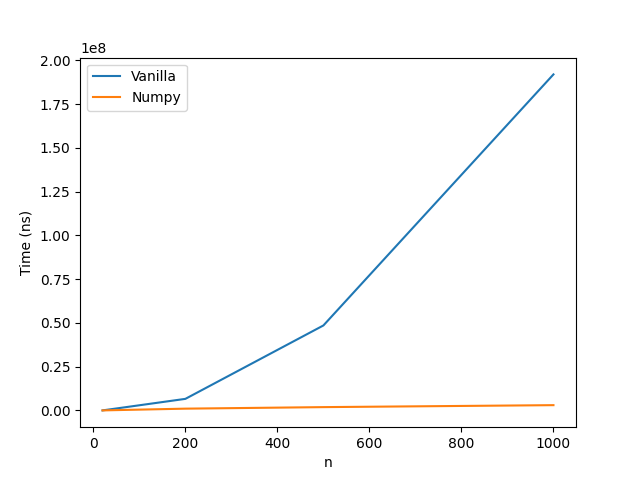
\includegraphics[width=4.5in]{./vanilla_vs_numpy_execution_time.png}
    \end{center}

    \medskip
    \textbf{Timing Data (3 runs):}

    \begin{center}
    \begin{tabular}{|c|c|c|c|c|}
    \hline
    \textbf{Run} & \textbf{n} & \textbf{Vanilla (ms)} & \textbf{NumPy (ms)} \\
    \hline
    \multirow{4}{*}{1} & small & 0.0 & 0.0 \\
    & & 6.5907 & 0.9986 \\
    & & 48.5399 & 1.8718 \\
    & large & 192.0126 & 2.9974 \\
    \hline
    \multirow{4}{*}{2} & small & 0.0 & 0.0 \\
    & & 8.065 & 0.9986 \\
    & & 49.9015 & 2.0058 \\
    & large & 200.7771 & 3.564 \\
    \hline
    \multirow{4}{*}{3} & small & 0.0 & 0.0 \\
    & & 13.704 & 0.0 \\
    & & 42.3925 & 0.0 \\
    & large & 195.6872 & 1.2134 \\
    \hline
    \end{tabular}
    \end{center}

    \medskip
    \textbf{Discussion:}

    Both implementations perform the same $O(n^2)$ work (matrix-vector multiplies, matrix addition). The algorithmic complexity is identical however vanilla Python's per-element interpreter overhead dominates at scale, while NumPy's compiled routines execute the same $O(n^2)$ work in optimized native code---in other words every multiplication or addition results in one call from Python to C code, whereas NumPy matrix operation is once per matrix operation. Underlying data structures used appear to be different as well, as the vanilla version uses Python lists, and the float objects are not guaranteed to be in contiguous blocks of memory, however NumPy arrays are stored contiguously resulting in better cache utilization.

\end{aprob}

\noindent\rule{\textwidth}{0.4pt}

\clearpage{}
\begin{aprob}
    Two random variables $X$ and $Y$ have equal  distributions if their CDFs, $F_X$ and $F_Y$, respectively, are equal, i.e. for all $x$, $ \abs{F_X(x) - F_Y(x)} = 0$. 
    The central limit theorem says that the sum of $k$ independent, zero-mean, variance $1/k$ random variables converges to a (standard) Normal distribution as $k$ tends to infinity.  
    We will study this phenomenon empirically (you will use the Python packages NumPy and Matplotlib).  Each of the following subproblems includes a description of how the plots were generated; these have been coded for you. The code is available in the .zip file. In this problem, you will add to our implementation to explore {\bf matplotlib} library, and how the solution depends on $n$ and $k$.
    
    \begin{enumerate}
    \item \points{2}  \label{prob:cltcdf:gaussian} For $i=1,\ldots,n$ let $Z_i \sim \mathcal{N}(0,1)$. Let $x\mapsto F(x)$ denote the true CDF from which each $Z_i$ is drawn (i.e.,  Gaussian). Define  $\widehat{F}_n(x) = \frac{1}{n} \sum_{i=1}^n \1\{ Z_i \leq x\}$ for $x\in\R$ and we will choose $n$ large enough such that, for all $x \in \R$,
    \[
        \sqrt{\E{\round{\widehat{F}_n(x)-F(x)}^2 }} \leq 0.0025\ .
    \]
    Plot $x\mapsto \widehat{F}_n(x)$ for $x$ ranging from $-3$ to $3$.
    
    \item  \points{2}  Define $Y^{(k)} = \frac{1}{\sqrt{k}} \sum_{i=1}^k B_i$ where each $B_i$ is equal to $-1$ and $1$ with equal probability and the $B_i$'s are independent.
    We know that each $\frac{1}{\sqrt{k}} B_i$ is zero-mean and has variance $1/k$. \label{prob:cltcdf:k} For each $k \in \set{1, 8, 64, 512}$ we will generate $n$ (same as in part a) independent copies $Y^{(k)}$ and plot their empirical CDF on the same plot as part~\ref{prob:cltcdf:gaussian}.
    \end{enumerate}
    Be sure to always label your axes. 
    Your plot should look something like the following (up to styling) (Tip: checkout \texttt{seaborn} for instantly better looking plots.)

    \begin{center}
        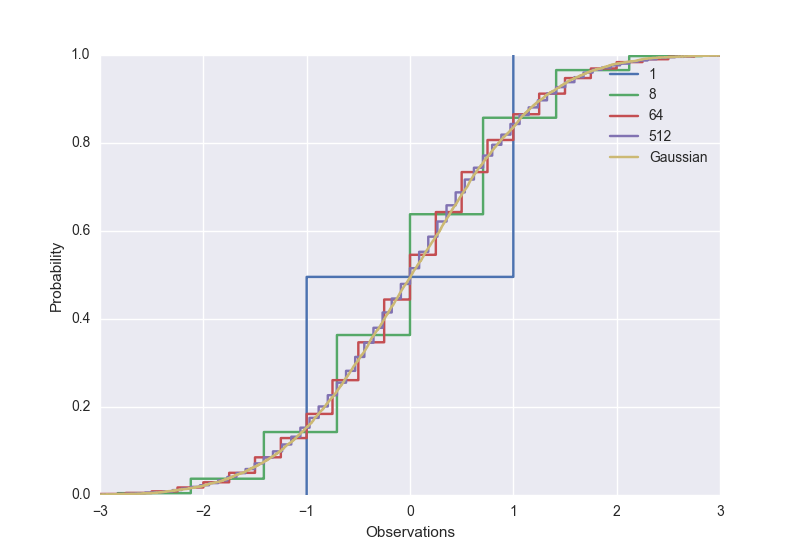
\includegraphics[width=4in]{./full.png}
    \end{center}
    
    \subsubsection*{What to Submit:}
    \begin{itemize}
        \item \textbf{Part~\ref{prob:cltcdf:gaussian}:} Value for $n$ (You can simply print the value determined by the code provided for you).
        \textbf{Part~\ref{prob:cltcdf:k}:} In 1-2 sentences: How does the empirical CDF change with $k$?
        \item \textbf{Parts~\ref{prob:cltcdf:gaussian} and~\ref{prob:cltcdf:k}:} Plot of $x\mapsto \widehat{F}_n(x)$ for $x \in [-3, 3]$
        \item \textbf{Code} on Gradescope through coding submission
    \end{itemize}
\end{aprob}

\clearpage{}
\appendix
\section*{Appendix: AI Collaboration Transcripts}

\subsection*{A1 --- Bayes' Theorem (chat\_conversation\_export\_A1.md)}

\begin{mdframed}
\textbf{User:} \\
After your yearly checkup, the doctor has bad news and good news. The bad news is that you tested positive for a serious disease, and that the test is 99\% accurate (i.e., the probability of testing positive given that you have the disease is 0.99, as is the probability of testing negative given that you don't have the disease). The good news is that this is a rare disease, striking only one in 10,000 people. What are the chances that you actually have the disease?

Please include links only don't describe the solution or the details of the concepts. I want to solve the problem after reading the material, don't solve the problem.

\bigskip
\textbf{Assistant:}
\begin{itemize}[leftmargin=*]
    \item \href{https://www.khanacademy.org/math/ap-statistics/probability-ap/stats-conditional-probability/a/tree-diagrams-conditional-probability}{Khan Academy --- Tree diagrams and conditional probability}
    \item \href{https://ocw.mit.edu/courses/18-05-introduction-to-probability-and-statistics-spring-2022/mit18_05_s22_lec03.pdf}{MIT OpenCourseWare --- Conditional Probability, Independence, Bayes' Theorem (18.05)}
    \item \href{https://ocw.mit.edu/courses/6-1200j-mathematics-for-computer-science-spring-2024/mit6_1200j_s24_lec19.pdf}{MIT OpenCourseWare --- Conditional Probability Lecture Notes (Mathematics for Computer Science)}
    \item \href{https://seeing-theory.brown.edu/}{Seeing Theory --- Bayesian Inference}
    \item \href{https://en.wikipedia.org/wiki/Conditional_probability}{Wikipedia --- Conditional probability}
    \item \href{https://en.wikipedia.org/wiki/Base_rate_fallacy}{Wikipedia --- Base rate fallacy}
\end{itemize}

\bigskip
\textbf{User:} \\
My intuition, look at false positive and true positives of a test in population and use that information to find out probability. Is that right direction? Don't solve the problem.

\bigskip
\textbf{Assistant:} \\
Yes. That is the right direction.

You want to think in terms of:
\begin{itemize}[leftmargin=*]
    \item how many people in a large population actually have the disease
    \item how many of those test positive
    \item how many people do \textbf{not} have the disease
    \item how many of those still test positive anyway
\end{itemize}

Then compare:
\begin{itemize}[leftmargin=*]
    \item \textbf{true positives}
\end{itemize}
against
\begin{itemize}[leftmargin=*]
    \item \textbf{all positives}
\end{itemize}

That framing is exactly the useful one here. Another good lens to review is \textbf{conditional probability / Bayes' theorem}, but your population-count intuition is often the cleanest way to reason it out.

\bigskip
\textbf{User:} \\
Download this chat conversation as an MD file.
\end{mdframed}

\subsection*{A2 --- Covariance Matrix (covariance\_matrix\_conversation\_A2.md)}

\begin{mdframed}
\textbf{User:} \\
Explain covariance matrix with 3 components/dimensions with a real world example.

\bigskip
\textbf{Assistant:} \\
Think of a covariance matrix as a compact way to describe how several quantities vary on their own and how they move together.

With \textbf{3 components}, the covariance matrix is a \textbf{3$\times$3 table}.

Let's use a real-world example:

Suppose you track, over many days, these 3 things for a delivery company:
\begin{itemize}[leftmargin=*]
    \item $X_1$: number of packages delivered
    \item $X_2$: fuel used
    \item $X_3$: driver overtime hours
\end{itemize}

Then the covariance matrix is:
\[
\boldsymbol\Sigma =
\begin{bmatrix}
\mathrm{Var}(X_1) & \mathrm{Cov}(X_1, X_2) & \mathrm{Cov}(X_1, X_3) \\
\mathrm{Cov}(X_2, X_1) & \mathrm{Var}(X_2) & \mathrm{Cov}(X_2, X_3) \\
\mathrm{Cov}(X_3, X_1) & \mathrm{Cov}(X_3, X_2) & \mathrm{Var}(X_3)
\end{bmatrix}
\]

\textbf{What each entry means:}

\textbf{Diagonal entries = variances} --- these tell you how much each variable fluctuates by itself.
\begin{itemize}[leftmargin=*]
    \item $\mathrm{Var}(X_1)$: how much package count changes from day to day
    \item $\mathrm{Var}(X_2)$: how much fuel usage changes
    \item $\mathrm{Var}(X_3)$: how much overtime changes
\end{itemize}
Big variance means that quantity is less stable.

\textbf{Off-diagonal entries = covariances} --- these tell you whether two variables tend to rise and fall together.
\begin{itemize}[leftmargin=*]
    \item $\mathrm{Cov}(X_1, X_2)$: when deliveries go up, does fuel use also go up?
    \item $\mathrm{Cov}(X_1, X_3)$: when deliveries go up, does overtime also increase?
    \item $\mathrm{Cov}(X_2, X_3)$: when fuel use is high, is overtime usually high too?
\end{itemize}

Interpretation:
\begin{itemize}[leftmargin=*]
    \item \textbf{Positive covariance}: they tend to increase together
    \item \textbf{Negative covariance}: when one goes up, the other tends to go down
    \item \textbf{Near zero covariance}: no clear linear relationship
\end{itemize}

\textbf{Example with numbers:}

Imagine the covariance matrix from your data is:
\[
\boldsymbol\Sigma =
\begin{bmatrix}
100 & 40 & 25 \\
40 & 64 & 20 \\
25 & 20 & 16
\end{bmatrix}
\]

Here is how to read it:
\begin{itemize}[leftmargin=*]
    \item \textbf{100}: package deliveries vary quite a bit
    \item \textbf{64}: fuel use also varies, but a little less
    \item \textbf{16}: overtime varies the least
\end{itemize}

And the relationships:
\begin{itemize}[leftmargin=*]
    \item \textbf{40} between deliveries and fuel: busier days usually use more fuel
    \item \textbf{25} between deliveries and overtime: more deliveries usually mean more overtime
    \item \textbf{20} between fuel and overtime: when routes are heavy enough to burn more fuel, overtime also tends to rise
\end{itemize}

\textbf{Why it is a matrix:}

Because with 3 variables, you need to describe each variable's own spread and each pairwise relationship. For 3 variables, that means 3 variances and 3 pairwise covariances. The matrix keeps all of that organized in one object.

\textbf{Geometric intuition:}

If you imagine each day as a point in 3D space (packages, fuel, overtime), then the covariance matrix tells you the \textbf{shape of the cloud of points}.
\begin{itemize}[leftmargin=*]
    \item Large variance in one direction $\rightarrow$ cloud spreads more along that axis
    \item Positive covariance between two variables $\rightarrow$ cloud tilts along those two axes
    \item Negative covariance $\rightarrow$ cloud tilts the opposite way
\end{itemize}

So the covariance matrix tells you both \textbf{how wide} the data is in each direction and \textbf{how tilted} the data is because variables move together.

\bigskip
\textbf{User:} \\
Export this conversation as an MD file.
\end{mdframed}

\subsection*{A3 --- Normal Distribution Properties (conversation\_export\_A3.md)}

\begin{mdframed}
\textbf{User:} \\
Can you provide pointers on concepts I should brush up on to solve these 4 problems? Including math basics.

Don't solve the problem give me pointers/links/youtube videos or freely available courses I should review.

\bigskip
\textbf{Assistant:} \\
Yes. For these four, I'd brush up in this order.

\textbf{1) Math basics first}
\begin{itemize}[leftmargin=*]
    \item \textbf{Sigma notation / summations}: you need to be comfortable reading expressions like $\frac{1}{n}\sum_{i=1}^n X_i$. Khan's summation review is a good quick refresher.
    \item \textbf{u-substitution for integrals}: part \textbf{b} explicitly hints at this, so make sure you can spot a substitution and change variables cleanly in definite or improper integrals. Khan and Paul's Online Notes are both solid.
\end{itemize}

\textbf{2) Core probability/statistics ideas}
\begin{itemize}[leftmargin=*]
    \item \textbf{Normal distribution basics}: mean $\mu$, variance $\sigma^2$, standardization, and what $\mathcal{N}(0,1)$ means. Khan's normal-distribution review/video or StatQuest are good for intuition.
    \item \textbf{Expectation and variance rules}: especially $\E{aX+b}$, $\Var{aX+b}$, $\E{X+Y}$, $\Var{X+Y}$, and when independence matters.
\end{itemize}

\textbf{3) What each part is really testing}
\begin{itemize}[leftmargin=*]
    \item \textbf{Part a}: linear transformation / standardization of a normal random variable. Review scaling and shifting of random variables.
    \item \textbf{Part b}: expected absolute value after standardization. That means normal pdf, symmetry, absolute value inside an expectation, and integration with substitution.
    \item \textbf{Part c}: linearity of expectation and variance of a linear combination of independent variables.
    \item \textbf{Part d}: sample mean / sampling distribution. You want to know the mean and variance of $\widehat{\mu}_n = \frac{1}{n}\sum X_i$, and then what multiplying by $\sqrt{n}$ does to mean and variance.
\end{itemize}

\textbf{4) Free resources}
\begin{itemize}[leftmargin=*]
    \item Khan Academy: statistics \& probability overview, then random variables, transformations, combining random variables, and sampling distributions.
    \item MIT OCW probability/statistics notes on expectation, variance, continuous random variables, and sums of independent normals.
    \item OpenStax \textit{Introductory Statistics 2e} for normal distributions and sampling distributions.
    \item StatQuest for normal distribution intuition.
\end{itemize}

\textbf{5) Tight study checklist}

Before attempting the problem set, make sure you can do these without notes:
\begin{itemize}[leftmargin=*]
    \item Read and manipulate sigma notation.
    \item Explain what happens to mean and variance under $Y = aX + b$.
    \item State when $\Var{X+Y} = \Var{X} + \Var{Y}$ is valid.
    \item Explain what the sample mean's distribution looks like when the $X_i$ are normal.
    \item Do a basic u-substitution cleanly.
\end{itemize}

If you want, I can turn this into a 30-minute targeted review plan in the exact order to study before you try the problems.

\bigskip
\textbf{User:} \\
Export this conversation as an MD file.
\end{mdframed}

\end{document}%